\documentclass[fleqn,final]{beamer}
\mode<presentation>
{
  \usetheme{ForumStatBlau}
}
\usepackage{times}
\usepackage{etex}
\usepackage{amsmath,amssymb}
%\usepackage{sfmath} % for sans serif math fonts; wget http://dtrx.de/od/tex/sfmath.sty
\usepackage[english]{babel}
\usepackage[ansinew]{inputenc}
\usepackage[orientation=portrait,size=a0,scale=1.25,debug]{beamerposter}
\usepackage{booktabs,array}
\usepackage{listings}
\usepackage{picins,graphicx}
\usepackage{xspace}
\usepackage{keyval}
\usepackage{listings}
\lstset{numbers=left,
	numberstyle=\tiny,
	numbersep=5pt,
	breaklines=true,
	showstringspaces=false,
	frame=l ,
	xleftmargin=15pt,
	xrightmargin=15pt,
	basicstyle=\ttfamily\scriptsize,
	stepnumber=1,
	%keywordstyle=\color{blue},          % keyword style
	commentstyle=\color{dkgreen},       % comment style
	stringstyle=\color{mauve},         % string literal style
	escapeinside={\%(}{\%}
}

\usepackage{wrapfig}
\usepackage{fp}
\usepackage{ifthen}
\usepackage[T1]{fontenc}
\usepackage{tikz,colortbl,pgf,pgfarrows,pgfnodes,pgfautomata,pgfheaps,pgfshade,eurosym, dsfont}

\usepackage{pgfplots}


\listfiles
\newcommand*{\signstream}{SignStream\texttrademark\xspace}
\newcommand{\WichtigFarbe}{\color{red}}%
\newcommand{\TextFarbe}{\color{black}}%


\def\bs{\boldsymbol}
\definecolor{darkblue}{rgb}{0.28,0,0.60}
\definecolor{hblue}{rgb}{0.70,0.7,1}
\definecolor{NR0}{rgb}{1,1,1}
\definecolor{NR1}{rgb}{1,1,0.8}
\definecolor{NR2}{rgb}{1,1,0.5}
\definecolor{NR3}{rgb}{1,1,0.25}
\definecolor{NR4}{rgb}{1,1,0.0}
\definecolor{NR5}{rgb}{1,0.75,0.0}
\definecolor{NR6}{rgb}{1,0.5,0.0}
\definecolor{NR7}{rgb}{1,0.25,0.0}
\definecolor{NR8}{rgb}{1,0,0.0}

\setbeamertemplate{navigation symbols}{}
\setbeamerfont{title}{series=\bfseries}


\setbeamerfont{frametitle}{series=\bfseries}
\setbeamertemplate{frametitle}
{
\begin{centering}
\insertframetitle\vspace*{-4mm}\par
\end{centering}
}

\newcommand{\convD}{\stackrel{\text{d}}{\longrightarrow}}
\newcommand{\E}{\text{E}\,}
\newcommand{\var}{\text{V}\,}



\title{\huge \textbf{emdi}: An R package for \textbf{E}stimating and \textbf{M}apping regional \textbf{D}isaggregated \textbf{I}ndicators} %konkreter Titel!!
\author{\large Ann-Kristin Kreutzmann, S�ren Pannier, Natalia Rojas-Perilla, Timo Schmid, Nikos Tzavidis \& Matthias Templ}
\institute{Freie Universit�t Berlin, University of Southampton \& Technische Universit�t Wien} % (optional, but mostly needed)

\date{today}


\begin{document}

\begin{frame}[fragile]{}
      
%%%%%%%%%%%%%%%%%%%%%%%%%%%%%%%%%%%%%%%%%%%%%%%%%%%%%%%%%%%%%%%%%%%%%%%%%%%%%%%%%
\vspace{-1cm} 
 \begin{columns}[t]
      \begin{column}{.50\linewidth}
        \begin{block}{\rule[-2.5mm]{0cm}{1cm}\textsc{Motivation}}


\begin{itemize}\small{

\item  The demand for indicators on a disaggregated level is increasing in order to improve policy decisions
\item Maps that combine the estimated indicators with geographical data are in favour for presenting these indicators 
\item User-friendly software tools can simplify the estimation of these indicators, the assessment of estimations and their visualization  

}

\end{itemize}


\end{block}
\vspace{-1cm}
%%%%%%%%%%%%%%%%%%%%%%%%%%%%%%%%%%
		

\vspace{-1.5cm}
        

  \end{column}
%%%%%%%%%%%%%%%%%%%%%%%%%%%%%%%%%%%%%%%%%%%%%%%%%%%%%%%%%%%%%%%%%%%%%%%%%%%%%%%%%


    \begin{column}{.47\linewidth}
		\begin{block}{\rule[-2.5mm]{0cm}{1cm}\textsc{Discussion and Outlook}}
			\vspace{-0.5cm}
			\small{
			    \begin{itemize}
						\item
						The package comprises all steps from estimation, assessment of estimation to presentation via maps and in excel 
						\item 
						It is especially simple to use the provided functions and thus to receive illustrative results
						\item
						\textbf{Further implementations:} More model-based small area estimation methods, a wider range of transformation methods and parallelization of the bootstrap computation
				  \end{itemize}
				}
		\end{block}

\end{column}
\end{columns}			
			
\begin{block}{\rule[-2.5mm]{0cm}{1cm}\textsc{How the R package emdi supports estimating and mapping disaggregated indicators}}
	\vspace*{-1.3cm}
\begin{columns}[t]
	\vspace*{0.3cm}
	\begin{column}{.28\linewidth}
		\begin{figure}
			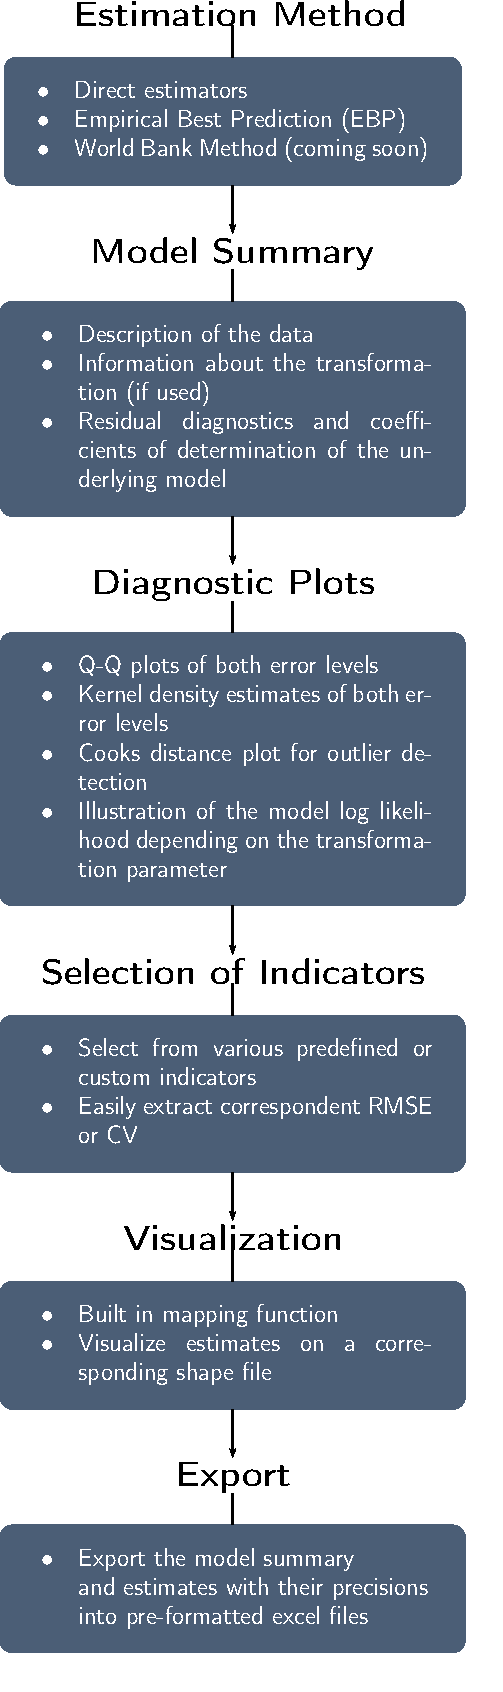
\includegraphics[width=22cm]{fluss_version1.pdf}
		\end{figure}	
	\end{column}
	
	
	\begin{column}{0.7\linewidth}
	

%%%%%%%%%%%%%%%%%%%%%%%%%%%%%%%%%%%%%%%%%%%%%%%%%%%%%%%%%%%%%%%%%%%%%%%%%
\vspace*{-1.3cm}
\begin{columns}[t]

	
	\begin{column}{0.58\linewidth}
		\small{
	\begin{block}{\rule[-0mm]{0cm}{0.5cm}\textsc{Receive point and MSE/variance estimates}}
			\begin{itemize}
				\item The direct estimates correspond to the direct estimates in the \textbf{laeken} package and thus comprise important poverty and inequality measures used in European and worldwide poverty and social exclusion analysis: Head Count Ratio, Poverty Gap, Gini coefficient and Quintile Share Ratio \\
				$\hookrightarrow$ \texttt{head\_count()}, \texttt{poverty\_gap()}, \texttt{gini()}, \texttt{quintile\_share()}
				\item The implemented model-based small area estimation method is the Empirical Best Prediction (EBP) approach by Molina and Rao (2010). For the EBP, the mentioned poverty and inequality indicators, the mean, and several quantiles (10\%, 25\%, median, 75\%, 90\%) are returned. Furthermore, the user can define multiple individual indicators by the argument \texttt{custom\_indicator}. \\
				$\hookrightarrow$ \texttt{ebp()} 
				\item Different transformations can be conducted in order to meet the Gaussian assumptions for model-based estimation methods: no transformation, log-transformation and Box-Cox transformation. For the latter, the optimal parameter is obtained by REML estimation.
			\end{itemize}	
	\end{block}
}
	{\small 			
		
		\begin{block}{\rule[-0mm]{0cm}{0.5cm}\textsc{Model diagnostics}}
			\vspace*{0.5cm}
			\begin{columns}
				\begin{column}{11cm}
					Graphical diagnostics contain the four graphs on the right and in case that Box-Cox transformation is used also the plot below.

					\begin{lstlisting}
					%( \textcolor{blue}{> plot(ebp)}%
					\end{lstlisting}
				\end{column}
				\hspace*{-2cm}
				\begin{column}{10cm}
						\begin{figure}
							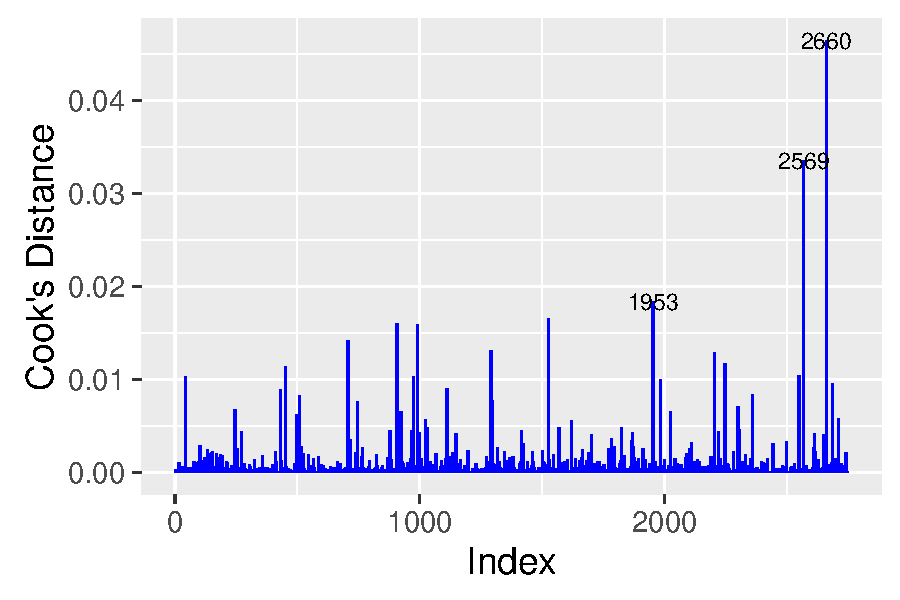
\includegraphics[width=10cm]{Graphics/cooks}
						\end{figure}
				\end{column}
				\begin{column}{10cm}
					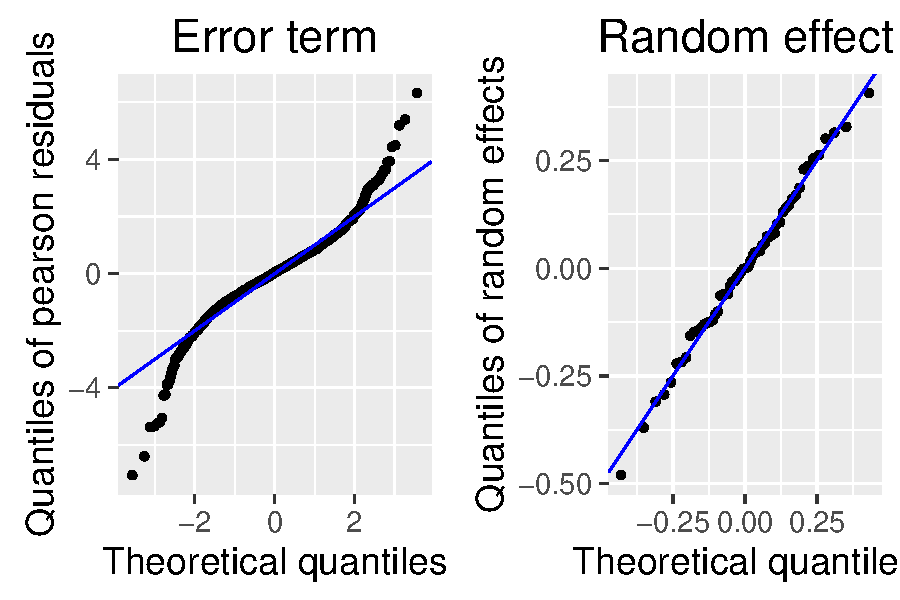
\includegraphics[width=10cm]{Graphics/qqplots}
				\end{column}
			\end{columns}
			\begin{figure}[t]
					\hspace*{-0.75cm}
			\begin{minipage}[hbt]{10cm}
	       		\raggedright
         		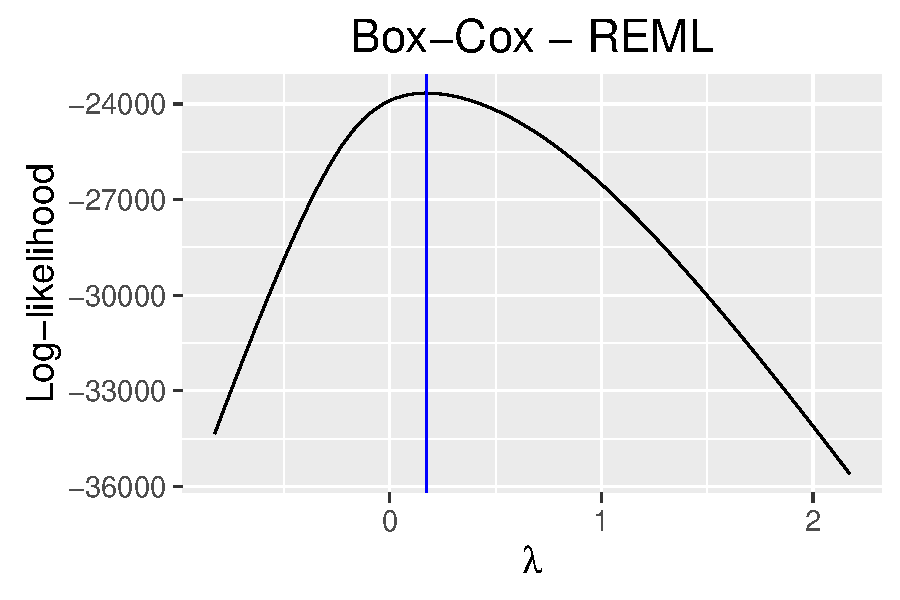
\includegraphics[width=10cm]{Graphics/optimal_lambda}
		     	\end{minipage}
		     	\hspace*{0.75cm}
				\begin{minipage}[hbt]{10cm}
					\centering
					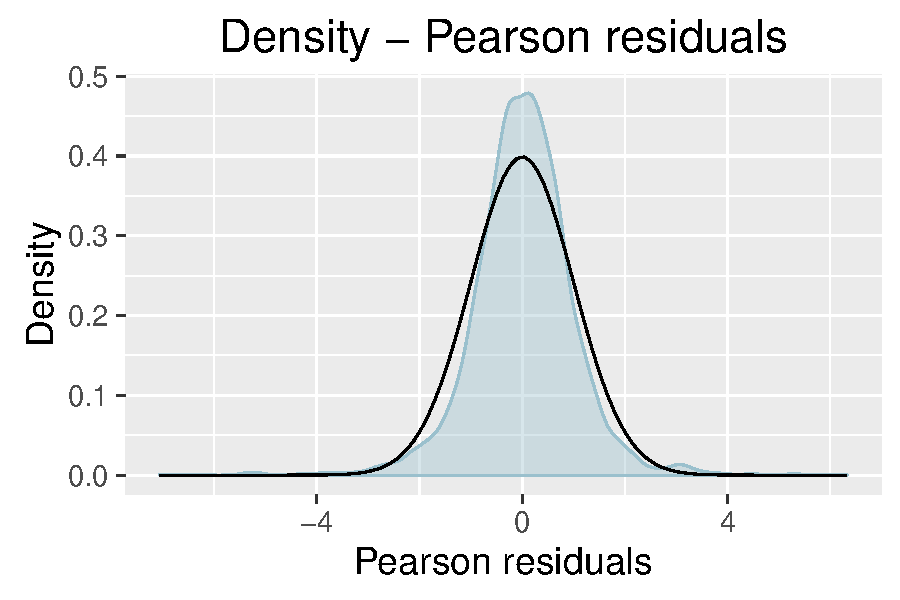
\includegraphics[width=10cm]{Graphics/density_res}
				\end{minipage}
				\hspace*{0.75cm}
				\begin{minipage}[hbt]{10cm}
					\centering
					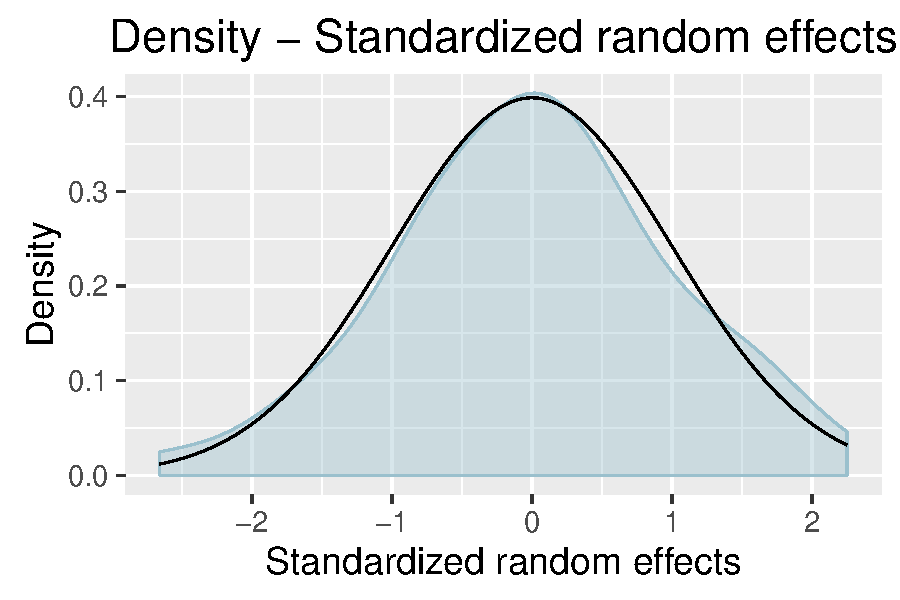
\includegraphics[width=10cm]{Graphics/density_re}
				\end{minipage}
			\end{figure}
		\end{block}
	}
\end{column}
\hspace*{0.1cm}
	\begin{column}{0.435\linewidth}
		\small{
			
			\begin{block}{\rule[-0mm]{0cm}{0.5cm}\textsc{Summarize estimation results}}
           	The \texttt{summary()} function gives information about the data sets, the data transformation, results of conducted normality checks and explanatory measures. Additionally, a summary especially of the underlying linear mixed model can be received by \texttt{summary(emdiObject\$model)}.
           	\vspace*{0.5cm}
				\begin{lstlisting}
				%( \textcolor{blue}{> summary(ebp)}%
				Empirical Best Prediction
				
				Call:
				ebp(fixed = ictpc ~ pcocup + jnived + clase_hog + pcpering + bienes + actcom,    
				   pop_data = census, pop_domains =            
				   "domain_id", smp_data = survey_mex, smp_domains =    
				   "domain_id", pov_line = 903.04, transformation = 
				   "box.cox", L = 50, MSE = T, B = 50, custom_indicator = list(my_max = function(y, pov_line) {max(y)}, my_min = function(y, pov_line) {min(y)}))
				
				Out-of-sample domains:  67 
				In-sample domains:  58 
				
				Sample sizes:
				Units in sample:  2748 
				Units in population:  219514 
				                   Min. 1st Qu. Median    Mean 3rd Qu.  Max.
				Sample_domains        3      17     21   47.38   42.25   527
				Population_domains  650     923   1161 1756.00 1447.00 13580
				
				Transformation:
				Transformation Method Optimal_lambda Shift_parameter
				       box.cox   reml       0.172312               1
				
				Explanatory measures:
				Marginal_R2 Conditional_R2
				0.4867911      0.4955212
				
				Residual diagnostics:
				                Skewness Kurtosis Shapiro_W    Shapiro_p
				Error         -0.2426125 7.951944 0.9500250 1.238856e-29
				Random_effect -0.1211658 3.003680 0.9936586 9.906020e-01
				
				ICC:  0.01701086 
				\end{lstlisting}
				
			\end{block}
		}
	\end{column}
	
\end{columns}
	
\vspace{-1cm}
\small{
\begin{block}{\rule[-0mm]{0cm}{0.5cm}\textsc{Select Indicators}}
	\begin{minipage}{13cm}
		Function \texttt{estimators()} enables to select \texttt{all} indicators, groups of indicators (\texttt{Poverty} and \texttt{Inequality}) and each indicator separately.
	\end{minipage}
	\hspace*{0.3cm}
\begin{minipage}{43cm}
	\begin{lstlisting}
	%( \textcolor{blue}{> estimators(object = ebp, MSE = T, CV = T, indicator = "Poverty")}%
	Indicator/s: Head_Count, Poverty_Gap
	                  Domain  Head_Count Head_Count_MSE Head_Count_CV Poverty_Gap Poverty_Gap_MSE Poverty_Gap_CV
	1                 Acambay 0.33861472   2.136365e-03    0.13649975  0.14101067    6.171988e-04     0.17618160
	2                 Acolman 0.18812822   9.045488e-04    0.15986818  0.06795016    1.620265e-04     0.18732794
	3                  Aculco 0.25606695   1.785476e-03    0.16501501  0.09855112    4.095351e-04     0.20534494
	4  Almoloya de Alquisiras 0.30166667   1.713125e-03    0.13720415  0.12177054    4.566486e-04     0.17548857
	5      Almoloya de Ju�rez 0.21157773   6.459450e-04    0.12012345  0.08261839    1.472854e-04     0.14689370
	6        Almoloya del R�o 0.18889381   8.946196e-04    0.15834396  0.07017192    1.947474e-04     0.19887149
	...
	\end{lstlisting}
\end{minipage}


	
	
	\vspace{-0.5cm}                                            
	
\end{block}    
}

\vspace{-0.7cm}
\small{
	\begin{block}{\rule[-0mm]{0cm}{0.5cm}\textsc{Map estimation results}}
 \begin{columns}
 	\hspace*{-1.5cm}
 	\begin{column}{.41\linewidth}
 	Function \texttt{map\_plot()} combines shape files with estimated indicators. If the domain variables differ between the data set and the shape file	a \texttt{data\_frame} that fits the variables is necessary.
 	\vspace*{0.2cm}
\begin{lstlisting}
map_table <- data.frame(Domain = unique(census$domain_id), 
                        mun = sort(shp_mex$mun))
%( \textcolor{blue}{> map\_plot(object = ebp, MSE = T, CV = T, map\_obj = shp\_mex,
indicator = "Head\_Count", map\_dom\_id = "mun", 
map\_tab = map\_table)}%
\end{lstlisting}
\end{column}
%%%%%%%%%%%%%%%%%%%%%%%%%%%%%%%%%%%%%%%%%%%%%%%%%%%%%%%%%%%%%%%%%%%%%%%%%%%%%%%%%
\hspace{-3.5cm}
	\begin{column}{.16\linewidth}
		\hspace*{-1.5cm}
		{\small 			
				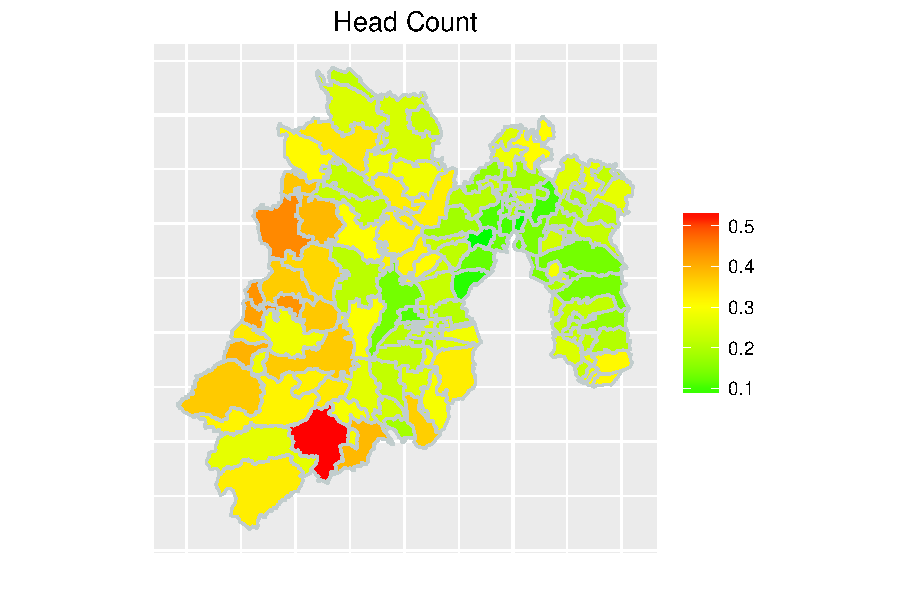
\includegraphics[height=10cm]{Graphics/point_hcr_map}	
		}
	\end{column}			
	
	\begin{column}{.16\linewidth}
		{\small 	
				\hspace*{-1.8cm}
				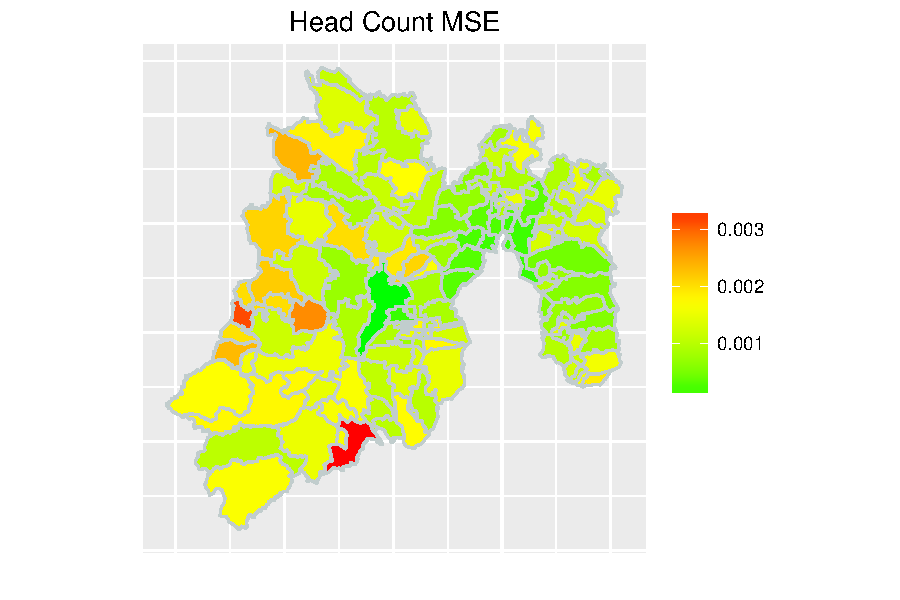
\includegraphics[height=10cm]{Graphics/mse_hcr_map}
		}
	\end{column}
	
	
	\begin{column}{.16\linewidth}
			\hspace*{-2.3cm}
		{\small
				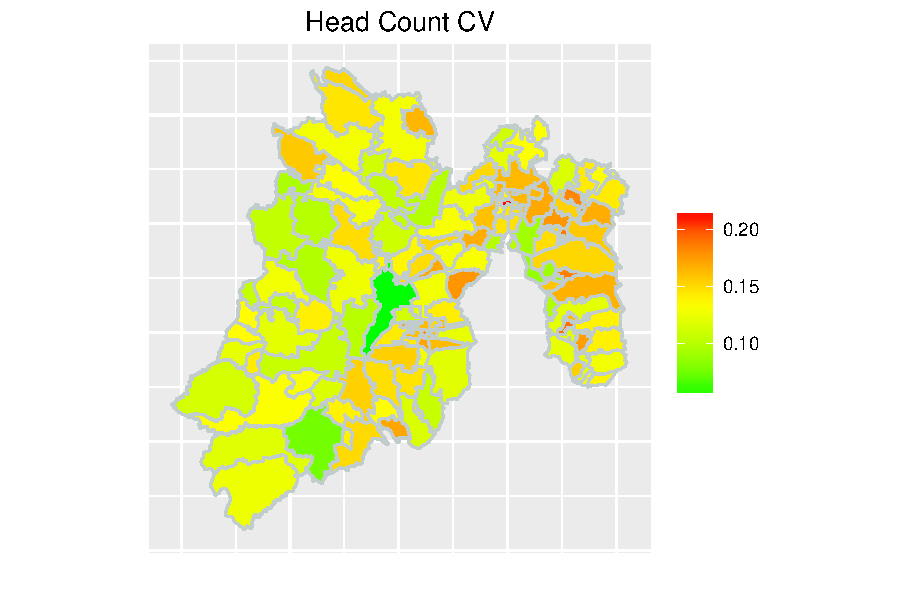
\includegraphics[height=10cm]{Graphics/cv_hcr_map}
		}
	\end{column}
\end{columns}


\end{block}	 
}	
\vspace{-1cm}



%%%%%%%%%%%%%%%%%%%%%%%%%%%%%%%%%%%%%%%%%%%%%%%%%%%%%%%%%%%%%%%%%%%%%%%%%%%%%%%%%%%%%%%%%%%%%%%%%%%%%%%%%%%%%%%%%%%%%%%%%%%%%%%%%%%%%%%%%%

\vspace*{-0.5cm}	
\small{ 	
\begin{block}{\rule[-0mm]{0cm}{0.5cm}\textsc{Export results to excel}}
\begin{columns}
	\vspace*{-2cm}
	\begin{column}{0.65\linewidth}
		Function \texttt{write\_excel()} enables to use the results independently of the statistical software R by exporting results to excel.
		\begin{lstlisting}
		%( \textcolor{blue}{> write.excel(ebp, file ="to\_excel.xlsx", indicator = "Poverty", MSE = T, CV = T)}%
		\end{lstlisting}
		\begin{figure}
			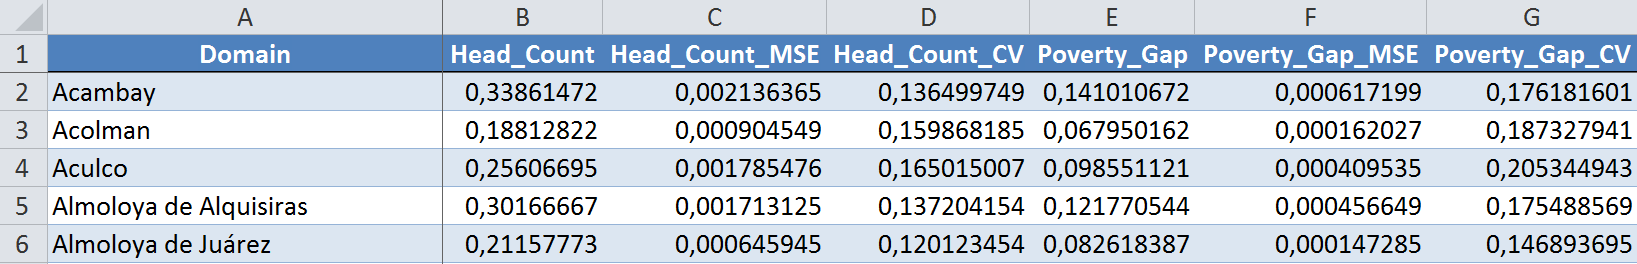
\includegraphics[height=6cm]{Graphics/estimates_excel}
		\end{figure}	
	\end{column}
	\begin{column}{0.35\linewidth}
		\begin{figure}
			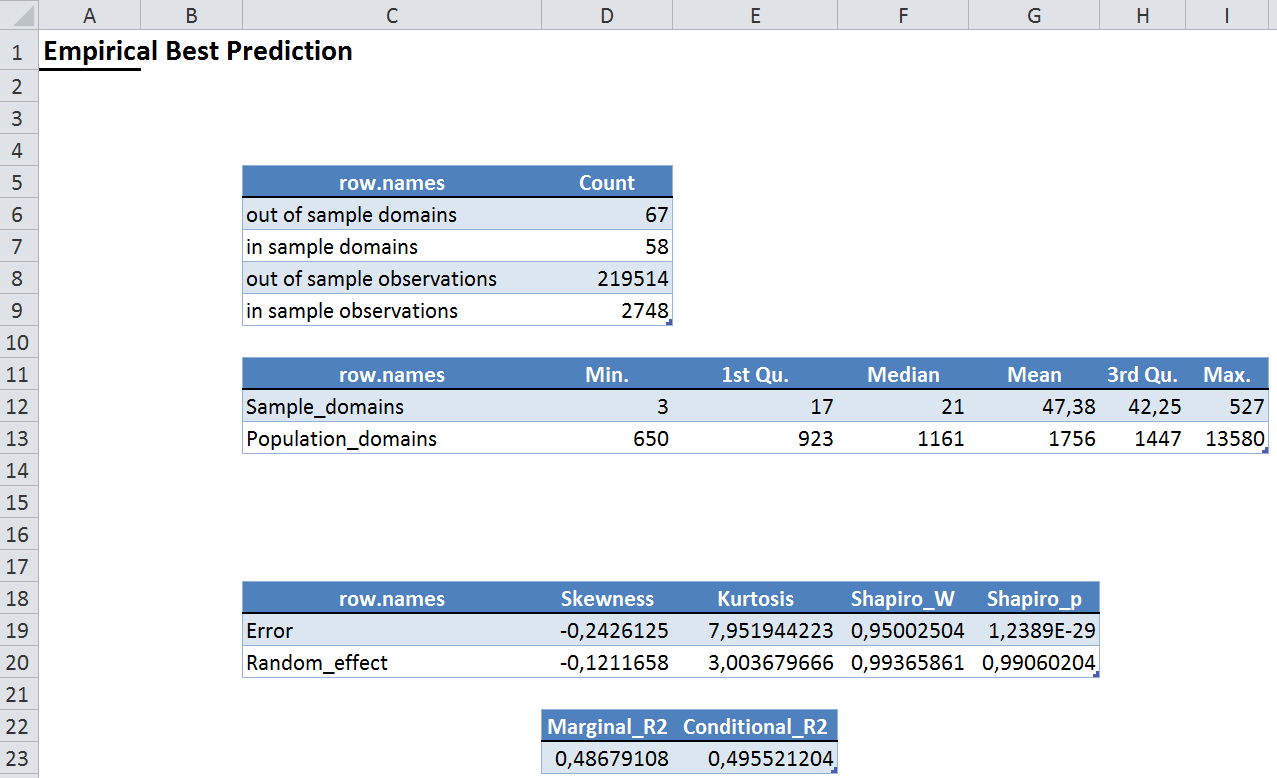
\includegraphics[width=17cm]{Graphics/summary_excel}
		\end{figure}
	\end{column}
\end{columns}

				





\end{block}	
} 	
%%%%%%%%%%%%%%%%%%%%%%%%%%%%%%%%%%%%%%%%%%%%%%%%%%%%%%%%%%%%%%%%%%%%%%%%%%%%%%%%%		
\end{column}
\end{columns}
\end{block}



\vspace{-1.8cm}
   \begin{block}{References}
   \vspace{-0.4cm}

\noindent [1] Alfons, A., \& Templ, M. (2013)
{\sl Estimation of Social Exclusion Indicators from Complex Surveys: The {R} Package {laeken}.\/} 
Journal of Statistical Software, 54(15), 1--25.\\

\noindent [2] Molina, I., \& Rao, J.N.K. (2010)
{\sl Small area estimation of poverty indicators.\/} 
Canadian Journal of Statistics, 38(3), 369--385.\\

\noindent [3]  Gurka, M. J., Edwards, L. J., Muller, K. E. \& Kupper, L. L. (2006)
{\sl Extending the Box--Cox Transformation to the Linear Mixed Model.\/}  Journal of the Royal Statistical Society. 26(2), 211--252.\\


    \end{block}

\end{frame}


\end{document}

